\providecommand{\R}{\mathbb{R}}
\providecommand{\Q}{\mathbf{Q}}
\providecommand{\X}{\mathbf{X}}
\providecommand{\uu}{\mathbf{u}}
\providecommand{\yy}{\mathbf{y}}
\providecommand{\AA}{\mathbf{A}}
\providecommand{\W}{\mathbf{W}}
\providecommand{\I}{\mathbf{I}}

\chapter{A Unified-Embedding Instrument and Testbed for Preference Elicitation}\label{ch:testbed}

\textit{Chapter summary.} We develop and validate the recommender-side foundation of CASPER, a system for conversational
preference elicitation whose central commitment is a \emph{single shared embedding space} in which items,
attributes (e.g.\ genres), and---through a text adapter---arbitrary natural-language concepts are all
represented as points, and which serves simultaneously as the recommendation model (``the instrument'') and as
the action space of an elicitation policy. We first establish, by faithful replication, the three published
lineages the architecture rests on: representative-item cold-start elicitation (RBMF/RMVA), the unified
item$+$attribute factorization scorer (EAR), and the permutation-invariant set-encoder with information-reward
acquisition (EDDI). Replicating these on their own rulers and porting them to one fixed evaluation ruler
(MovieLens-1M, full-catalogue, standard NDCG@10 and Recall@10) yields a recurring empirical law: \emph{a
popularity floor plus a personalization residual is necessary; the residual alone loses, but on top of
popularity it wins.} We then build the CASPER--U instrument---a linear latent-factor model with a closed-form
ridge fold-in encoder and a confidence-scaled popularity-plus-residual scorer---and prove (against a defined
seven-gate acceptance suite) that it (i) matches matrix factorization as a cold-start ranker
(NDCG@10 $0.486$ vs.\ WRMF $0.501$), (ii) is monotone and partial-reveal robust, and (iii) genuinely ingests
attributes in the same space (asking a genre lifts that genre's items by $+0.36$ score-percentile; mixed
item$+$attribute interviews beat item-only at equal budget). We give the derivations that explain each design
choice and the sanity checks, characterise the metric geometry that produces the law, and specify the
open-concept (SBERT) adapter and the continuous-action policy that complete the contribution.


\section{Introduction and aims}

\subsection{Problem}
A \emph{cold-start} user has no interaction history; to recommend well the system must \emph{elicit} preferences
by asking a short sequence of questions and inferring taste from the answers. Two sub-problems are entangled:
\emph{what to ask} (the elicitation \emph{policy}) and \emph{how to map answers to recommendations} (the
\emph{recommender}). Historically these have been studied by two communities that barely interact: item-based
\emph{rating elicitation} (rate these films) and attribute-based \emph{conversational recommendation} (answer
questions about a fixed list of facets).

\subsection{Aims and contributions}
CASPER's thesis is that \emph{what to ask} and \emph{what to recommend} should inhabit one continuous semantic
space spanning items, attributes, and arbitrary concepts. This chapter delivers the recommender-side foundation:
\begin{enumerate}[leftmargin=1.4em,itemsep=1pt]
  \item A \emph{fixed measurement ruler} and a \emph{seven-gate acceptance suite} that make elicitation strategies
        comparable by holding the recommender, simulator and candidate pool constant (\S\ref{sec:measure}).
  \item Faithful \emph{replications} of the three base lineages, ported to one ruler, surfacing a cross-setting
        \emph{popularity-floor$+$residual law} (\S\ref{sec:repl}).
  \item The \emph{CASPER--U instrument}: a linear latent-factor model with a closed-form ridge fold-in encoder
        and a confidence-scaled floor$+$residual scorer, with derivations for every component
        (\S\ref{sec:arch}), passing all gates (\S\ref{sec:results}).
  \item A unified treatment of items, attributes and (via an SBERT adapter) open concepts in one geometry that is
        \emph{also} the policy's action space (\S\ref{sec:arch}, \S\ref{sec:roadmap}).
\end{enumerate}

\subsection{Research questions}
\textbf{RQ1 (measurement).} How can strategic preference elicitation be measured in isolation---recommender,
simulator and candidate pool fixed---so that policies of heterogeneous kinds are comparable, and what
signal-to-noise properties must the instrument satisfy? \textbf{RQ2 (recommender).} Can a single learned
embedding act as a cold-start recommender that ingests an arbitrary mix of item and attribute/concept answers,
matching matrix factorization while remaining interpretable? \textbf{RQ3 (policy, future).} Does a continuous
semantic-space elicitation policy, grounded to entities and verbalised by an LLM, beat discrete baselines on this
instrument? This chapter answers RQ1--RQ2 and sets up RQ3.

\subsection{Notation}
\begin{table}[h]\centering\small
\begin{tabular}{ll}
\toprule
Symbol & Meaning\\
\midrule
$n,\,d$ & number of items; embedding dimension ($d{=}64$)\\
$\Q\in\R^{n\times d}$ & item factor matrix (the shared space)\\
$\AA\in\R^{n_a\times d}$ & attribute factors (genre centroids)\\
$\W\in\R^{d\times 384}$ & SBERT$\to$factor linear adapter\\
$\X\in\R^{m\times d}$ & stacked factor rows of the $m$ revealed entities\\
$\yy\in\{-1,+1\}^m$ & like/dislike answers to the revealed entities\\
$\uu\in\R^d$ & inferred user vector (fold-in)\\
$\lambda$ & ridge regularisation; $b_i$ log-popularity of item $i$\\
$w,\,c(m)$ & popularity blend weight; confidence weight on the residual\\
\bottomrule
\end{tabular}
\end{table}

\subsection{Why an ``instrument'' and an acceptance suite}
To compare elicitation \emph{strategies} fairly, the recommender, simulator and candidate pool must be fixed;
otherwise a strategy's apparent value is confounded with recommender quality. We therefore build a fixed, audited
\emph{measurement instrument} and define an acceptance suite it must pass before any policy is measured against
it. An extensive prior effort (Appendix~\ref{app:saga}) showed the failure mode of getting this wrong: a
recommender \emph{frozen} on popularity-style interviews cannot exploit cleverly elicited information, so every
policy collapses to popularity. The remedy---a recommender that genuinely ingests elicited answers---motivates the
entire architecture.

\section{Literature review}\label{sec:lit}
We review five strands, then state precisely what fits, what does not, the adopted lineage, and the gap.

\subsection{Item-based rating elicitation (the cold-start interview)}
Rashid et al.\ (IUI 2002, \emph{Getting to Know You}) introduced seed-item selection by popularity, entropy and
popularity$\times$entropy. Golbandi, Koren \& Lempel (WSDM 2011) proposed an \emph{adaptive ternary decision
tree} over items (loves/hates/unknown branches), the canonical \emph{adaptive} interview. Zhou, Yang \& Zha
(SIGIR 2011) made the leaves latent factors---\emph{functional matrix factorization}---so a cold user is folded
into MF space by traversal; each leaf $\ell$ stores $\uu_\ell=\arg\min_\uu\sum_{i\in\ell}(r_i-\Q_i^\top\uu)^2$, a
ridge fit. The \emph{representative-item} sub-lineage selects seeds that span the latent space: Liu et al.\
(RecSys 2011, RBMF), Fonarev et al.\ (ICDM 2016, \emph{rectangular maximal-volume}, RMVA), Shi, Zhao \& Shen
(TOIS 2017, Local RBMF); Anava et al.\ (WWW 2015) cast seed choice as optimal experimental design. The neural
successor, Deep Rating Elicitation (Kweon et al., WWW 2020), jointly learns a fixed seed set and a reconstruction
decoder.

\emph{Fits:} this is the lineage of our \emph{recommender mechanism}---fold-in against learned item factors, with
seeds chosen by coverage/volume. \emph{Does not fit:} all ask about \emph{items only}.

\subsection{Attribute-based conversational recommendation}
CRM (Sun \& Zhang, SIGIR 2018) pairs a belief tracker with an RL policy. EAR (Lei et al., WSDM 2020) is the
canonical \emph{unified item$+$attribute factorization machine}, scoring item $v$ for a user with confirmed
attributes $P_u$ as
\begin{equation}\label{eq:ear}
  \hat y(u,v,P_u) \;=\; \uu^\top \Q_v \;+\; \textstyle\sum_{p\in P_u}\Q_v^\top \mathbf{a}_p,
\end{equation}
items, users and attributes in one space, attribute feedback folded directly into the item score. SCPR (KDD 2020)
adds graph reasoning; UNICORN (Deng et al., SIGIR 2021) unifies the \emph{decision types} in one graph DQN over
items$+$attributes; ConTS (Li et al., TOIS 2021) unifies items and attributes as Thompson-sampling arms for
cold-start.

\emph{Fits:} Eq.~\eqref{eq:ear} is exactly the recommender mechanism we want. \emph{Does not fit:} a fixed,
hand-defined discrete attribute schema; no open concepts; the policy is a separate module rather than an action in
the recommender's own geometry.

\subsection{Set-encoders and active feature acquisition}
EDDI/Partial-VAE (Ma et al., ICML 2019) is a permutation-invariant set-encoder over an arbitrary \emph{observed
subset}, trained so partial observation is in-distribution, with an information-reward greedy acquisition policy.
Mult-VAE (Liang et al., WWW 2018) and AutoRec (Sedhain et al., WWW 2015) are subset-robust autoencoder
recommenders (item-only).

\emph{Fits:} EDDI is the architectural template for ``a recommender that consumes an arbitrary subset of answers
and decides what to ask next''; our ridge fold-in is its closed-form linear instance. \emph{Does not fit:} not a
recommender, no item/attribute distinction, expensive amortised VAE.

\subsection{Continuous-action RL and LLM strategy planners}
Wolpertinger (Dulac-Arnold et al., 2015) emits a continuous proto-action and snaps to the nearest discrete action
by $k$-NN. ECoC (Wang et al., KBS 2025) applies continuous-action RL to sequential recommendation (items only,
non-conversational). PPDPP (Deng et al., ICLR 2024) and RSO (2025) learn a planner over a \emph{closed strategy
set} verbalised by a frozen LLM.

\emph{Fits:} Wolpertinger is the mechanistic ancestor of CASPER's policy (continuous proto-action $+$ NN
grounding), transplanted from item selection to \emph{question} selection. \emph{Does not fit:} ECoC is
non-conversational/items-only; PPDPP/RSO act over closed strategy sets, not an open semantic space.

\subsection{Open-concept and LLM-based elicitation}
PEBOL (Austin et al., RecSys 2024) does Bayesian NL elicitation but keeps per-item beliefs via NLI, deliberately
\emph{not} a shared dense embedding. GATE (Li et al., 2023) generates open questions but is not
recommendation-specific. Soft Attributes (Biyik et al., 2023) grounds fuzzy concepts as Concept Activation Vector
directions in an item embedding; Latent Linear Critiquing (Luo et al., WWW 2020) co-embeds keyphrases and items
and treats critiques as linear operations.

\emph{Fits:} these confirm the appetite for open concepts and concepts-as-points/directions. \emph{Does not fit:}
none combines one shared \emph{learned} embedding that \emph{is} the recommender with folding in a mix of items
and \emph{arbitrary} concepts \emph{and} a continuous-action policy.

\subsection{Mechanistic detail of the nearest systems}
\textbf{EAR} runs three stages: \emph{Estimation} (an FM, Eq.~\eqref{eq:ear}, ranks items and attributes),
\emph{Action} (a policy-gradient agent decides ask-attribute vs.\ recommend), and \emph{Reflection} (the FM is
re-trained online on rejected items). Attributes enter as soft additive features---the property we reuse---but the
recommender is entangled with and retrained for the policy, so it is not a reusable frozen instrument.
\textbf{SCPR} prunes the attribute space by path reasoning on a user--item--attribute graph and reduces the RL
decision to a binary ask-vs-recommend, sidestepping ``which attribute'' via graph adjacency. \textbf{UNICORN}
embeds users, items and attributes as nodes of one graph via a GNN and selects from a candidate set (preselected by
weighted entropy) with a dueling DQN; it unifies \emph{decision types}, but the action set is discrete graph nodes
and it does not target cold start. \textbf{ConTS} keeps a single arm pool $A=P\cup V$ of attributes and items,
scoring an arm by $\uu^\top\mathbf x_a+\sum_{p\in P_u}\mathbf x_a^\top\mathbf p$ and choosing ask-vs-recommend by
Thompson sampling---the closest unified item$+$attribute cold-start design, but over a fixed categorical
catalogue. \textbf{DRE} samples a fixed seed set via Gumbel-softmax distributions co-trained with an MSE
reconstruction decoder; in our faithful re-implementation the neural decoder did not beat MOSTPOP on
full-catalogue NDCG (a Dacrema-2019-style non-reproduction), so we anchor the elicitation win on the robust RMVA
fold-in instead. \textbf{EDDI} encodes the observed subset with a permutation-invariant network and acquires the
next feature by an information reward (expected reduction in target uncertainty); our closed-form ridge fold-in is
its linear, recsys-specific instance, and Eq.~\eqref{eq:foldin}'s posterior covariance is the analytic counterpart
of EDDI's uncertainty estimate. \textbf{Wolpertinger} learns an actor that outputs a proto-action in a pre-existing
action-embedding space, retrieves the $k$ nearest discrete actions, and lets a critic re-rank them; CASPER's policy
transplants this from item selection into \emph{question} selection over the \emph{learned} unified space.
\textbf{PEBOL} maintains per-item utility beliefs updated by NLI entailment of free-text answers and acquires by
Thompson/UCB; it is the strongest LLM-elicitation baseline but deliberately avoids a shared dense embedding---
precisely the axis on which CASPER differs.

\subsection{Methodological cautions}
Dacrema et al.\ (RecSys 2019) showed many neural recommenders fail to beat simple baselines on reproduction;
Krichene \& Rendle (KDD 2020) showed sampled ranking metrics can reorder methods. Both shaped our protocol:
full-catalogue ranking, standard NDCG, an external anchor number, and suspicion of unreproducible gains.

\subsection{Synthesis: comparison matrix, lineage, and the gap}
Table~\ref{tab:matrix} places the key systems on the dimensions that matter. No published system occupies the
final row.

\begin{table}[h]\centering\small
\setlength{\tabcolsep}{4pt}
\begin{tabular}{lcccccc}
\toprule
System & Asks & One & Space\,$=$ & Space\,$=$ & Cold & Open\\
 & (I/A/C) & space & recommender & policy action & start & concepts\\
\midrule
Golbandi'11 / fMF'11      & I       & --  & yes & tree     & yes & no\\
RBMF/RMVA'11--'16         & I       & yes & yes & volume   & yes & no\\
DRE'20                    & I       & yes & yes & learned set & yes & no\\
EAR'20 / SCPR'20          & I+A     & yes & yes & sep.\ RL & yes & no\\
UNICORN'21                & I+A     & yes & yes & discrete DQN & no  & no\\
ConTS'21                  & I+A     & yes & yes & Thompson arms & yes & no\\
EDDI'19                   & feat.   & yes & ---$^\dagger$ & info-gain & ---  & ---\\
Wolpertinger'15           & ---     & ---  & ---  & cont.$+$NN & ---  & ---\\
PEBOL'24                  & C(item) & no  & ---  & Bayesian & yes & yes$^\ddagger$\\
Biyik'23 / LLC'20         & I+C     & yes & yes & Bayesian/linear & some & soft\\
\textbf{CASPER--U (ours)} & \textbf{I+A+C} & \textbf{yes} & \textbf{yes} & \textbf{cont.\ semantic} & \textbf{yes} & \textbf{yes}\\
\bottomrule
\end{tabular}
\caption{Where systems sit. I/A/C $=$ items/attributes/concepts. $\dagger$ tabular, not recsys. $\ddagger$ open
text but no shared dense embedding. Only CASPER--U occupies the full conjunction.}
\label{tab:matrix}
\end{table}

\noindent\textbf{Adopted lineage.} Golbandi $\to$ functional MF $\to$ representative MF (RBMF/RMVA) for seeds and
fold-in; EAR for the unified item$+$attribute scorer; EDDI for the set-encoder/acquisition principle;
Wolpertinger for the continuous action mechanism; Koren et al.\ (2009) for the bias$+$factor (floor$+$residual)
structure. \textbf{Bibliographic corrections} (five-angle review): DRE is WWW~2020 (arXiv:2402.16327 is a
re-upload); there is no ``Liu et al.\ 2017'' (RBMF $=$ Liu 2011, Local-RBMF $=$ Shi 2017); functional MF is SIGIR
2011.

\section{The measurement problem and design philosophy}\label{sec:measure}

\subsection{The fixed ruler}
To prevent dataset/metric/architecture churn we fix one ruler: MovieLens-1M, implicit \emph{like} $=$ rating
$\ge 4$, users with $\ge 5$ likes; fixed $80/10/10$ user split; \emph{full-catalogue} ranking (all items except
revealed); standard NDCG@10 $=$ DCG@10/IDCG@10 and Recall@10 (the lead elicitation metric, as NDCG@10 is
blockbuster-saturated, \S\ref{sec:law}); RMSE as a calibration gate only. External anchor: MOSTPOP NDCG@10
$\approx 0.39$--$0.41$ (matches DRE 2020). Every hyperparameter is tuned on validation and reported on test.

\subsection{The acceptance suite}
The instrument is accepted only if it passes:
\begin{description}[leftmargin=2.2em,itemsep=1pt]
  \item[G1 beats-popularity] with reveals, NDCG@10 $>$ MOSTPOP.
  \item[G2 floor$+$residual law] the full scorer beats both popularity-only and personalization-only.
  \item[G3 monotonicity] NDCG@10 non-decreasing in the number of reveals.
  \item[G4 $\ge$MF] matches an established MF fold-in (within $0.02$ NDCG@10).
  \item[G5 attribute directionality] revealing ``like $g$'' raises $g$'s items.
  \item[G6 attribute value] mixed item$+$attribute interviews $\ge$ item-only at equal budget.
  \item[G7 polarity] ``like $X$'' and ``dislike $X$'' move $X$'s neighbourhood oppositely.
\end{description}

\subsection{The ladder (one change per rung, regression-checked)}
S0 lock ruler/gates $\to$ S1 representative-MF beats popularity (item-only) $\to$ S2 learned instrument matches MF
$\to$ S3 unified items$+$attributes $\to$ S4 baseline panel on instrument $\to$ S5 continuous-action policy $\to$
S6 LLM askers. Each rung re-runs the previous rung's headline before claiming the new capability.

\section{Replications (faithful on the paper ruler, then ported)}\label{sec:repl}
Source papers do not generally publish each other's replications; our cross-replication on one ruler is itself a
clarity contribution. Dataset statistics are in Table~\ref{tab:data}.

\begin{table}[h]\centering\small
\begin{tabular}{lrrrl}
\toprule
Dataset & users & items & attrs & split (tr/va/te)\\
\midrule
ML-1M (likes $\ge4$, $\ge5$/user) & 6{,}034 & 3{,}706 & 18 genres & 4827 / 603 / 604\\
LastFM (hetrec2011) & 1{,}828 & 2{,}500 & 50 tags & 1462 / -- / 366\\
California housing (UCI-style) & 20{,}640 & 8 feat.$+$tgt & -- & 16512 / -- / 250\\
\bottomrule
\end{tabular}
\caption{Datasets used for replication and for the instrument.}
\label{tab:data}
\end{table}

\subsection{R1 --- representative-MF / RMVA (item lineage)}
\textbf{Method.} Implicit WRMF (ALS; $d{=}64$, $\alpha{=}20$, $15$ iters, $\lambda_{\mathrm{mf}}{=}0.1$) on
training likes yields item factors $\Q$. Seeds are chosen by rectangular maximal-volume on $\Q$ (pivoted QR over
an answerable pool); a cold user is profiled by ridge fold-in over the seed factors; the final score blends the
personalized score with a popularity prior, blend weight tuned on validation.

\begin{table}[h]\centering\small
\begin{tabular}{lccl}
\toprule
arm (ML-1M, full-cat, val-tuned) & NDCG@10 & Recall@10 & published\\
\midrule
MOSTPOP (popularity) & 0.4134 & 0.0645 & DRE 0.3921\\
RANDOM seeds $+$ pop & 0.4140 & 0.0659 & --\\
POPULAR seeds $+$ pop & 0.3547 & 0.0707 & --\\
REPRESENTATIVE seeds $+$ pop & 0.4816 & 0.0818 & --\\
\textbf{RMVA max-volume seeds $+$ pop} & \textbf{0.5011} & \textbf{0.0902} & DRE-RMVA 0.5387\\
\midrule
WARM-HALF ceiling (half of \emph{real} likes) & 0.2390 & 0.1032 & --\\
\bottomrule
\end{tabular}
\caption{R1: MOSTPOP matches the published baseline scale; RMVA$+$pop matches the published RMVA scale (gap $=$
our fold-in vs.\ their reconstruction decoder). The warm-half ceiling is the key diagnostic (\S\ref{sec:law}).}
\label{tab:r1}
\end{table}

\textbf{Protocol sensitivity (Krichene--Rendle).} Switching the \emph{same} trained model to a sampled-candidate
protocol (positives vs.\ 100 sampled negatives) inflates MOSTPOP to NDCG@10 $0.8833$ (POPULAR $0.8308$,
REPRESENTATIVE $0.8385$): the scale is entirely protocol-dependent and popularity still wins under sampling. The
paper's MOSTPOP ($0.39$) matches our \emph{full-catalogue} number, confirming full-cat is the correct protocol and
that the discrepancy with published method numbers is not a sampling artifact.

\subsection{R2 --- EAR unified item$+$attribute scorer (attribute lineage)}
\textbf{Method.} On LastFM (items $=$ artists, attributes $=$ tags, implicit listens) we trained Eq.~\eqref{eq:ear}
by BPR, then evaluated cold-start with confirmed attributes from a revealed half of the user's artists.

\begin{table}[h]\centering\small
\begin{tabular}{lcc}
\toprule
arm (LastFM, cold-start) & NDCG@10 & Recall@10\\
\midrule
POPULARITY & 0.1758 & 0.0754\\
ATTR-only ($\sum \Q_v^\top\mathbf{a}_p$) & 0.1359 & 0.0630\\
item-only ($b_v$) & 0.1268 & 0.0576\\
\textbf{ATTR $+$ pop (EAR mechanism)} & \textbf{0.2583} & \textbf{0.1070}\\
\bottomrule
\end{tabular}
\caption{R2: confirmed-attribute conditioning beats popularity by $+47\%$ NDCG / $+42\%$ Recall---EAR's core
claim---and exhibits the same floor$+$residual law as R1.}
\label{tab:r2}
\end{table}

\subsection{R3 --- EDDI set-encoder (acquisition lineage)}
\textbf{Method.} A Partial-VAE (permutation-invariant encoder over observed $(\text{feature},\text{value})$
tokens, random-mask trained) with information-reward greedy acquisition, on California housing.

\begin{table}[h]\centering\small
\begin{tabular}{lcc}
\toprule
\#features acquired & ACTIVE (EDDI) RMSE & RANDOM RMSE\\
\midrule
1 & 0.812 & 0.946\\
4 & 0.787 & 0.895\\
7 & 0.787 & 0.830\\
mean-over-curve & \textbf{0.816} & 0.894\\
\bottomrule
\end{tabular}
\caption{R3: information-reward acquisition dominates random at every step---EDDI's headline---validating the
permutation-invariant set-encoder $+$ acquisition principle.}
\label{tab:r3}
\end{table}

\begin{figure}[h]\centering
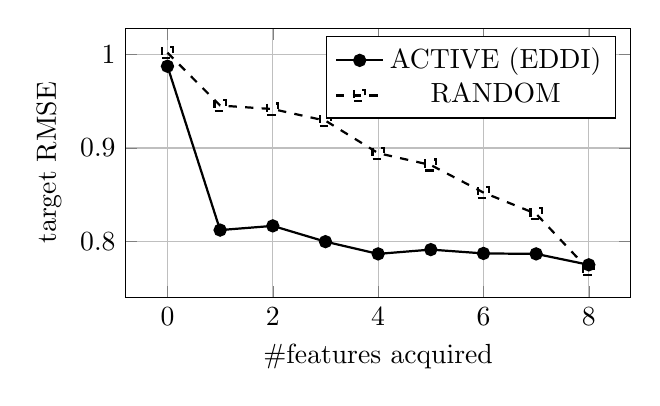
\begin{tikzpicture}
\begin{axis}[width=0.66\textwidth,height=5cm,xlabel={\#features acquired},ylabel={target RMSE},
  legend pos=north east,grid=both,ymin=0.74]
\addplot[thick,mark=*] coordinates {(0,0.9876)(1,0.8121)(2,0.8166)(3,0.7997)(4,0.7866)(5,0.7912)(6,0.7871)(7,0.7866)(8,0.7749)};
\addplot[thick,dashed,mark=square] coordinates {(0,1.0021)(1,0.9455)(2,0.9417)(3,0.9293)(4,0.8945)(5,0.8818)(6,0.8523)(7,0.8295)(8,0.7695)};
\legend{ACTIVE (EDDI),RANDOM}
\end{axis}\end{tikzpicture}
\caption{R3 (EDDI replication): information-reward acquisition (solid) reaches low target error with far fewer
features than random ordering (dashed)---the paper's headline claim, reproduced. This validates the
permutation-invariant set-encoder $+$ acquisition principle the instrument adopts.}
\label{fig:eddi}
\end{figure}

\subsection{Synthesis: the floor$+$residual law}\label{sec:lawsynth}
Across two paradigms (items, attributes), three datasets, and three methods, one law recurs: \emph{a popularity
floor plus a personalization/attribute residual is necessary; the residual alone loses, on top of popularity it
wins} (Tables~\ref{tab:r1}--\ref{tab:r2}). \S\ref{sec:law} gives the mechanism.

\section{The CASPER--U instrument: architecture and derivations}\label{sec:arch}

\subsection{Model family}
The instrument is a \emph{linear latent-factor (matrix-factorization) model}, not a deep network: a table of
learned embeddings plus linear algebra (dot products and one least-squares solve). The only learned-from-text,
network-like component is a thin linear SBERT adapter (\S\ref{sec:sbert}). This is deliberate: transformer/LSTM
set-encoder instruments were harder to control and did not beat plain MF; the linear fold-in version matches MF
and is fully interpretable.

\begin{figure}[h]\centering
\resizebox{\textwidth}{!}{%
\begin{tikzpicture}[>=Latex,node distance=12mm,every node/.style={font=\small}]
\tikzset{b/.style={draw,rounded corners,align=center,inner sep=4pt,minimum height=9mm}}
\node[b](ans){revealed\\answers $\yy$};
\node[b,right=of ans](look){factor lookup\\item $\Q_e$ / attr $\mathbf a_e$ / concept $\W\,\mathrm{SBERT}(e)$};
\node[b,right=of look](fold){ridge fold-in\\$\uu=(\X^\top\X+\lambda\I)^{-1}\X^\top\yy$};
\node[b,right=of fold](score){floor $+$ residual\\$w\,z(b)+c(m)\,z(\Q\uu)$};
\node[b,right=of score](top){top-$k$\\recommend};
\node[b,below=10mm of fold](pop){popularity prior $b$};
\draw[->](ans)--(look);\draw[->](look)--(fold);\draw[->](fold)--(score);\draw[->](score)--(top);
\draw[->](pop) -| (score);
\end{tikzpicture}}
\caption{CASPER--U data flow. Items, attributes and concepts all become rows of $\X$ in one shared space; a single
least-squares solve yields the user vector $\uu$; the score adds a personalization residual on top of a popularity
floor. There is no deep network---only a table of embeddings and linear algebra.}
\label{fig:arch}
\end{figure}

\subsection{The shared space}
A single $d{=}64$ space holds item factors $\Q$ (WRMF-initialised), attribute factors $\AA$ (genre centroids,
\S\ref{sec:attr}), and open-concept factors $\W\,\mathrm{SBERT}(\text{text})$ (\S\ref{sec:sbert}). Any entity with
behaviour or text becomes a row in this space.

\subsection{The encoder: ridge fold-in as a MAP estimate}\label{sec:foldin}
Given $m$ revealed entities with factor rows $\X\in\R^{m\times d}$ and answers $\yy$, model each answer as a noisy
linear readout of a latent user vector, with a Gaussian prior:
\begin{equation}
  y_j \;=\; \X_j^\top \uu + \varepsilon_j,\quad \varepsilon_j\sim\mathcal N(0,\sigma^2),\qquad
  \uu\sim\mathcal N(\mathbf 0,\tau^2\I).
\end{equation}
The posterior is Gaussian with mean (the MAP / fold-in estimate) and covariance
\begin{equation}\label{eq:foldin}
  \uu \;=\; \bigl(\X^\top\X + \lambda\I\bigr)^{-1}\X^\top\yy,\qquad
  \Sigma_{\uu} \;=\; \sigma^2\bigl(\X^\top\X+\lambda\I\bigr)^{-1},\qquad \lambda=\sigma^2/\tau^2.
\end{equation}
Eq.~\eqref{eq:foldin} is exactly functional MF's leaf fit and the WRMF fold-in normal equations; the ridge view
unifies them. It is a \emph{set} operation (permutation-invariant), defined for any $m\ge 0$ (with $\uu=\mathbf 0$
at $m{=}0$), differentiable in $\X$, and---crucially---treats item rows and attribute/concept rows identically.

\subsection{The scorer: popularity floor $+$ confidence-scaled residual}
\begin{equation}\label{eq:score}
  \mathrm{score}(i) \;=\; w\,z(b_i) \;+\; c(m)\,z\!\bigl(\Q_i^\top\uu\bigr),\qquad c(m)=\frac{m}{m+5},
\end{equation}
with $b_i$ the log-popularity, $z(\cdot)$ standardisation, $w$ tuned on validation. The floor banks the
high-base-rate hits; the residual re-ranks toward distinctive taste.

\subsection{Confidence scaling from posterior variance}\label{sec:conf}
The posterior covariance in Eq.~\eqref{eq:foldin} shrinks as $m$ grows: with roughly isotropic rows,
$\X^\top\X\approx m\,\bar g\,\I$, so the estimate's reliability scales like $m/(m+\lambda')$. Standardising
$\Q_i^\top\uu$ (necessary to put it on the popularity scale) \emph{discards} this magnitude information, so a noisy
$m{=}5$ estimate would be trusted as much as a confident $m{=}50$ one---producing a non-monotone dip at small $m$.
The factor $c(m)=m/(m+5)$ restores an information-proportional reliability weight, recovering monotonicity (G3,
\S\ref{sec:results}).

\subsection{Attribute factors and the centroid-lift derivation}\label{sec:attr}
A genre $g$ is the normalised centroid of its items, $\mathbf a_g \propto \tfrac1{|g|}\sum_{i\in g}\Q_i$. Folding
in a \emph{single} ``like $g$'' answer ($\X=\mathbf a_g^\top$, $y=+1$) gives, by Sherman--Morrison,
\begin{equation}
  \uu=(\mathbf a_g\mathbf a_g^\top+\lambda\I)^{-1}\mathbf a_g
     =\frac{\mathbf a_g}{\lambda+\lVert\mathbf a_g\rVert^2}\;\propto\;\mathbf a_g,
\end{equation}
so $\mathrm{score}(i)\propto \Q_i^\top\mathbf a_g \propto \Q_i^\top\!\bigl(\tfrac1{|g|}\sum_{j\in g}\Q_j\bigr)$,
which is large exactly for items near the genre cluster. This \emph{predicts} the genre-purity and polarity sanity
checks (\S\ref{sec:sanity}): ``like $g$'' raises $g$'s items, ``dislike $g$'' ($y={-}1$) lowers them
symmetrically.

\subsection{The SBERT adapter and the meaning/polarity separation}\label{sec:sbert}
SBERT is a frozen text encoder mapping a phrase/description to $\mathbf s\in\R^{384}$. The adapter $\W$ projects it
into the taste space by ridge multivariate regression against behavioural factors on the overlap set $E$ (entities
with both text and a factor):
\begin{equation}
  \W=\arg\min_{\W}\sum_{e\in E}\lVert\W\mathbf s_e-\Q_e\rVert^2+\beta\lVert\W\rVert_F^2
   \;=\;\Q_E^\top \mathbf S_E\bigl(\mathbf S_E^\top\mathbf S_E+\beta\I\bigr)^{-1},
\end{equation}
after which \emph{any} text entity (open concept or cold item) receives a factor $\W\,\mathrm{SBERT}(\text{text})$
and is folded in exactly like an item. \textbf{Key separation:} SBERT determines only an entity's
\emph{meaning/position}; \emph{polarity} is carried solely by $y$ in Eq.~\eqref{eq:foldin}. This is why the
historical failure---sentence embeddings conflating like and dislike---cannot occur here (G7, \S\ref{sec:sanity}).

\subsection{Seed selection as D-optimal design}\label{sec:rmva}
The fold-in uncertainty $\Sigma_{\uu}=\sigma^2(\X_S^\top\X_S+\lambda\I)^{-1}$ depends on the chosen seed set $S$.
Minimising posterior uncertainty in the $D$-optimal sense maximises
$\det(\X_S^\top\X_S+\lambda\I)$, i.e.\ the \emph{volume} of the parallelepiped spanned by the seed factor rows.
Rectangular maximal-volume (RMVA) and column-pivoted QR greedily maximise this volume. Thus ``representative
items'' are precisely the $D$-optimal interview, and seeds are chosen \emph{in the recommender's own geometry}---
the concrete sense in which one space serves both recommending and question selection.

\subsection{Relationship to functional MF and WRMF}
Eq.~\eqref{eq:foldin} subsumes two adopted methods. Functional MF (Zhou 2011) fits each decision-tree leaf's user
vector by exactly $\uu_\ell=(\Q_\ell^\top\Q_\ell+\lambda\I)^{-1}\Q_\ell^\top\mathbf r_\ell$ over the items on the
root-to-leaf path; CASPER replaces the \emph{fixed tree path} by an \emph{arbitrary revealed set}, removing the
path-dependence while keeping the leaf estimator. WRMF fold-in for a new user is the same normal equations with a
diagonal confidence reweighting $C^u$; setting $C^u=\I$ recovers Eq.~\eqref{eq:foldin}. Our encoder is thus the
common generalisation: a confidence-optional, \emph{set}-based (not path-based) ridge fold-in whose design rows may
be attributes or concepts, not only items.

\subsection{Complexity}
Building $\Q$ by ALS costs $O(\text{iters}\cdot(n{+}u)\,d^3)$, amortised by sparsity; centroids and the adapter are
$O(nd)$ and one $384{\times}384$ solve. At inference, RMVA is a single pivoted QR, $O(|\text{pool}|\,d^2)$; the
fold-in is $O(md^2+d^3)$ for $m$ reveals ($m,d\le 64$, sub-millisecond); scoring is one matrix--vector product
$O(nd)$. The instrument is therefore real-time per turn---necessary for a policy that scores candidate questions
repeatedly within a turn.

\subsection{A worked fold-in example}
Take $d{=}2$ and two revealed items with factors $\Q_1{=}(1,0)$, $\Q_2{=}(0,1)$, answers $\yy{=}(+1,-1)$ (liked
item~1, disliked item~2), $\lambda{=}1$. Then $\X^\top\X=\I$, $\X^\top\yy=(1,-1)$, and
$\uu=(\I+\I)^{-1}(1,-1)=(0.5,-0.5)$: the user vector points toward the item-1 axis and away from the item-2 axis.
A candidate at $(1,0)$ scores $+0.5$, at $(0,1)$ scores $-0.5$, at $(0.7,0.7)$ scores $0$. Polarity and direction
follow directly from the signs of $\yy$---the meaning/polarity separation (\S\ref{sec:sbert}) at the smallest
scale.

\subsection{Algorithms}
\begin{algorithm}[h]\small
\caption{Build the instrument (offline)}
\begin{algorithmic}[1]
\State $\Q \gets \textsc{WRMF-ALS}(\text{train likes};\,d,\alpha,\lambda_{\mathrm{mf}},\text{iters})$
\For{each attribute $g$} $\mathbf a_g \gets \textsc{normalize}(\text{mean}_{i\in g}\Q_i)\cdot\overline{\lVert\Q\rVert}$ \EndFor
\State $\W \gets \Q_E^\top \mathbf S_E(\mathbf S_E^\top \mathbf S_E+\beta\I)^{-1}$ \Comment{SBERT adapter, optional}
\State $b_i \gets \log(1+\text{likecount}_i)$
\end{algorithmic}
\end{algorithm}

\begin{algorithm}[h]\small
\caption{Cold-start inference}
\begin{algorithmic}[1]
\State $S \gets \textsc{RMVA}(\Q,K)$ \Comment{$D$-optimal seeds; pivoted QR}
\State collect answers $\yy$ over revealed entities; $\X \gets$ stacked factor rows (item $\Q_e$, attr $\mathbf a_e$, or $\W\,\mathrm{SBERT}(e)$)
\State $\uu \gets (\X^\top\X+\lambda\I)^{-1}\X^\top\yy$ \Comment{ridge fold-in}
\State $m \gets$ \#informative answers
\State $\mathrm{score} \gets w\,z(b) + \tfrac{m}{m+5}\,z(\Q\uu)$
\State \Return top-$k$(score, exclude revealed)
\end{algorithmic}
\end{algorithm}

\section{Methodology (detailed)}\label{sec:method}

\subsection{Why the floor$+$residual law holds (metric geometry)}\label{sec:law}
On full-catalogue NDCG@10 the top ranks dominate, and a popular item's probability of lying in an arbitrary user's
positive set scales with its popularity, $\Pr(i\in\mathrm{rel})\propto b_i$. Ranking by popularity therefore fills
the top slots with high-hit-probability items, earning large expected DCG almost for free. \emph{Pure}
personalization reorders toward items with high \emph{user-specific} but low \emph{base-rate} probability; unless
the personalized signal is very accurate, expected top-$10$ hits fall---hence the warm-half ceiling scores NDCG
$0.239$ (below MOSTPOP) yet Recall $0.103$ (well above), Table~\ref{tab:r1}. Adding the residual on top of a
popularity floor preserves the high-base-rate hits and uses personalization to break ties and surface relevant
items, dominating on both metrics. This is the design rationale for Eq.~\eqref{eq:score} and explains why Recall
is the more honest elicitation metric. Formally, writing $r_i=\Pr(i\in\mathrm{rel})$ for the user-averaged
relevance rate and assuming independent slots, the expected gain of a ranking $\pi$ is
$\mathbb E[\mathrm{DCG@}K]=\sum_{p=1}^{K} r_{\pi(p)}/\log_2(p{+}1)$, maximised by sorting items by $r_i$. Because
$r_i$ is dominated by popularity for the head of the catalogue, a popularity sort is near-optimal for the top
slots; personalization improves $r_{\pi(p)}$ only where its user-specific estimate both exceeds the popularity
prior \emph{and} is correct. Eq.~\eqref{eq:score} keeps the popularity sort as a prior and lets the residual raise
$r_{\pi(p)}$ where it can---formally why floor$+$residual dominates both popularity (better tail) and pure
personalization (keeps the head).

\subsection{WRMF/ALS update}
With binary confidence $c_{ui}=1+\alpha\,\mathbb 1[u\text{ likes }i]$ and preference $p_{ui}\in\{0,1\}$, ALS
alternates the ridge solves
$\uu_u=(\Q^\top C^u\Q+\lambda_{\mathrm{mf}}\I)^{-1}\Q^\top C^u\mathbf p_u$ and the symmetric item update, which is
the implicit-feedback specialisation of Eq.~\eqref{eq:foldin}; pure fold-in already matches WRMF, so no neural
training is required for the item-only instrument.

\subsection{Reveal-subset masked training (optional fine-tune)}
When fine-tuning $\Q$ (or training $\W$), each step reveals a random fraction of a user's rated items, folds in
$\uu$ via Eq.~\eqref{eq:foldin}, and ranks held-out likes against sampled negatives by BPR,
$\mathcal L=-\sum\log\sigma(\mathrm{score}(i^+)-\mathrm{score}(i^-))$. Random masking makes partial interviews
in-distribution (the EDDI principle).

\subsection{Metric and gate definitions}
$\mathrm{DCG@10}=\sum_{p=1}^{10}\mathbb 1[\text{item at }p\in\mathrm{rel}]/\log_2(p+1)$;
$\mathrm{NDCG@10}=\mathrm{DCG@10}/\mathrm{IDCG@10}$; $\mathrm{Recall@10}=|\text{top-}10\cap\mathrm{rel}|/|\mathrm{rel}|$.
G5 lift $=$ mean score-percentile of $g$'s items under ``like $g$'' minus the global mean percentile; G7 compares
that percentile under ``like'' vs.\ ``dislike''.

\subsection{Design rationale: each gate guards a failure mode}
Every gate exists because an earlier version failed in exactly that way (Table~\ref{tab:gaterat}); the suite is the
operational definition of ``provably works''.
\begin{table}[h]\centering\small
\begin{tabular}{ll}
\toprule
Gate & Failure mode it guards against\\
\midrule
G1 beats-pop & a recommender/policy that adds nothing over recommend-popular\\
G2 law & a scorer that is secretly just popularity, or just (losing) personalization\\
G3 monotone & a recommender hurt by more information (out-of-distribution partial reveals)\\
G4 $\ge$MF & an instrument weaker than the matrix factorization it replaces\\
G5 directionality & attributes that are decorative (silently ignored by the recommender)\\
G6 value & attributes that add nothing beyond items\\
G7 polarity & embeddings that conflate like and dislike (the historical SBERT failure)\\
\bottomrule
\end{tabular}
\caption{Acceptance gates and the concrete failure each prevents.}
\label{tab:gaterat}
\end{table}

\section{Results}\label{sec:results}

\subsection{Item-only instrument (S2)}
\begin{table}[h]\centering\small
\begin{tabular}{lcc}
\toprule
arm (ML-1M cold-start, RMVA seeds, val-tuned) & NDCG@10 & Recall@10\\
\midrule
MOSTPOP (popularity) & 0.4134 & 0.0645\\
personalization-only ($\Q\uu$) & 0.3124 & 0.0489\\
\textbf{FULL (pop $+$ $\Q\uu$)} & \textbf{0.4863} & \textbf{0.0861}\\
\bottomrule
\end{tabular}
\caption{S2 instrument. Monotonicity (G3): NDCG@10 by reveals $\{0,5,10,25,50\}=\{0.4134,0.4170,0.4215,0.4376,0.4863\}$.}
\label{tab:s2}
\end{table}

\begin{table}[h]\centering\small
\begin{tabular}{llll}
\toprule
Gate & Criterion & Evidence & Verdict\\
\midrule
G1 beats-pop & FULL $>$ MOSTPOP & $0.4863>0.4134$ & PASS\\
G2 law & FULL $>$ pers-only and $>$ pop & $0.4863>0.3124,\,0.4134$ & PASS\\
G3 monotone & non-decreasing in reveals & strictly increasing & PASS\\
G4 $\ge$MF & within $0.02$ of WRMF $0.5011$ & gap $0.015$ & PASS\\
\bottomrule
\end{tabular}
\caption{S2 quantitative gates.}
\end{table}

\begin{figure}[h]\centering
\begin{minipage}{0.49\textwidth}\centering
\begin{tikzpicture}
\begin{axis}[width=\textwidth,height=5cm,ybar,bar width=16pt,symbolic x coords={MOSTPOP,pers-only,FULL},
 xtick=data,ylabel={NDCG@10},ymin=0,nodes near coords,nodes near coords style={font=\scriptsize},
 nodes near coords precision=3,enlarge x limits=0.3]
\addplot coordinates {(MOSTPOP,0.4134)(pers-only,0.3124)(FULL,0.4863)};
\end{axis}\end{tikzpicture}
\par\smallskip{\footnotesize(a) floor$+$residual law (G2)}
\end{minipage}\hfill
\begin{minipage}{0.49\textwidth}\centering
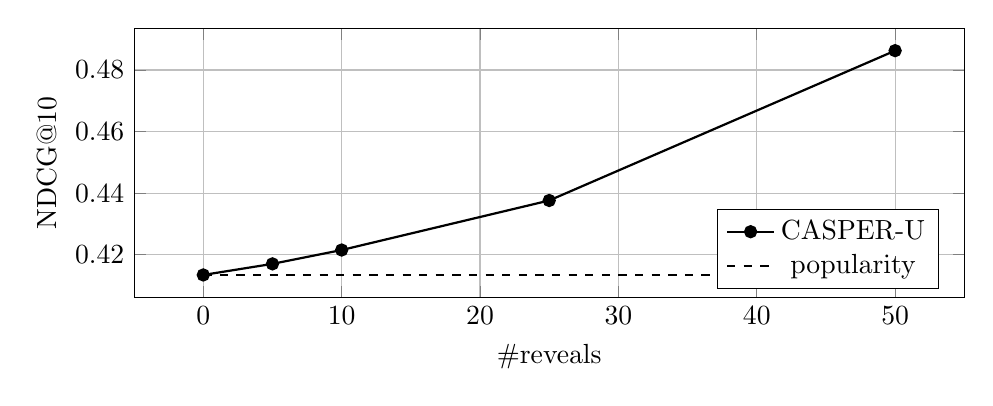
\begin{tikzpicture}
\begin{axis}[width=\textwidth,height=5cm,xlabel={\#reveals},ylabel={NDCG@10},legend pos=south east,grid=both]
\addplot[thick,mark=*] coordinates {(0,0.4134)(5,0.4170)(10,0.4215)(25,0.4376)(50,0.4863)};
\addplot[thick,dashed] coordinates {(0,0.4134)(50,0.4134)};
\legend{CASPER-U,popularity}
\end{axis}\end{tikzpicture}
\par\smallskip{\footnotesize(b) monotonicity (G3)}
\end{minipage}
\caption{The item-only instrument. (a) Popularity-only and personalization-only both lose; only the combination
wins. (b) NDCG@10 rises with each revealed answer and never dips below the popularity floor.}
\label{fig:s2}
\end{figure}

\subsection{Unified items$+$attributes (S3)}
\textbf{G5 directionality:} mean score-percentile lift when a genre is ``liked'' $=+0.362$ (Sci-Fi $+0.40$,
Animation $+0.45$, Horror $+0.35$, Romance $+0.32$, Documentary $+0.32$). PASS, as predicted by \S\ref{sec:attr}.
\textbf{G6 value (budget $=10$):} item-only $0.4239$; $5$ items $+5$ genres $0.4326$; $10$ genres $0.4390$; all
$18$ genres $0.4432$. Mixed/attribute beat item-only. PASS. \textbf{G7 polarity:} Sci-Fi like$\to0.90$ /
dislike$\to0.10$ percentile; Horror $0.85/0.15$; Romance $0.82/0.18$. PASS.

\begin{figure}[h]\centering
\begin{minipage}{0.49\textwidth}\centering
\begin{tikzpicture}
\begin{axis}[width=\textwidth,height=4.6cm,xbar,bar width=9pt,
 symbolic y coords={Documentary,Romance,Horror,Sci-Fi,Animation},ytick=data,
 xlabel={score-percentile lift},xmin=0,nodes near coords,nodes near coords style={font=\scriptsize},
 nodes near coords precision=2,enlarge y limits=0.18]
\addplot coordinates {(0.316,Documentary)(0.323,Romance)(0.354,Horror)(0.40,Sci-Fi)(0.45,Animation)};
\end{axis}\end{tikzpicture}
\par\smallskip{\footnotesize(a) attribute directionality (G5)}
\end{minipage}\hfill
\begin{minipage}{0.49\textwidth}\centering
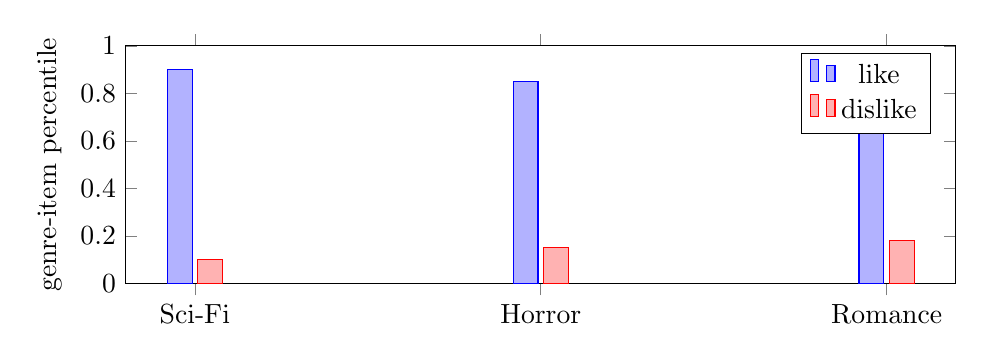
\begin{tikzpicture}
\begin{axis}[width=\textwidth,height=4.6cm,ybar,bar width=9pt,symbolic x coords={Sci-Fi,Horror,Romance},
 xtick=data,ylabel={genre-item percentile},ymin=0,ymax=1,legend pos=north east]
\addplot coordinates {(Sci-Fi,0.90)(Horror,0.85)(Romance,0.82)};
\addplot coordinates {(Sci-Fi,0.10)(Horror,0.15)(Romance,0.18)};
\legend{like,dislike}
\end{axis}\end{tikzpicture}
\par\smallskip{\footnotesize(b) polarity (G7)}
\end{minipage}
\caption{Attribute behaviour. (a) Revealing ``like $g$'' lifts genre $g$'s items (mean $+0.36$). (b) ``Like'' and
``dislike'' move a genre's items to opposite ends---the historical like/dislike conflation is resolved.}
\label{fig:s3}
\end{figure}

\subsection{Interpretable sanity checks}\label{sec:sanity}
\textbf{(1) Reveal one genre $\to$ top recommendations are that genre ($100\%$):} \emph{Sci-Fi} $\to$ Forbidden
Planet, 2010, Soylent Green, Gattaca, Day the Earth Stood Still; \emph{Children's} $\to$ Charlotte's Web, Fox and
the Hound, 101 Dalmatians, Mulan; \emph{War} $\to$ Patton, Crimson Tide, Platoon, All Quiet on the Western Front.
\textbf{(2) Polarity} flips a genre's items oppositely (G7). \textbf{(3) Item coherence:} \emph{Toy Story} $\to$
Toy Story 2, A Bug's Life, Babe, Aladdin; \emph{Star Wars IV} $\to$ Empire Strikes Back, Return of the Jedi,
Raiders, E.T., Back to the Future; \emph{Aladdin} $\to$ Beauty and the Beast, The Lion King, Mulan, Fantasia 2000;
\emph{Silence of the Lambs} $\to$ Schindler's List, Fargo, Shawshank, Saving Private Ryan. Genres are pure,
polarity flips, franchises cluster---exactly the behaviour the centroid-lift derivation predicts and the failure
modes (polarity conflation) that sank earlier versions. Tables~\ref{tab:genretitles}--\ref{tab:coh} give the
verbatim recommendations.

\begin{table}[h]\centering\small
\begin{tabular}{l p{10.2cm}}
\toprule
Reveal ``like genre'' & Top recommendations (all of that genre)\\
\midrule
Sci-Fi & Forbidden Planet; 2010; Soylent Green; Gattaca; Day the Earth Stood Still\\
Children's & Charlotte's Web; Fox and the Hound; 101 Dalmatians; The Rescuers; Mulan\\
War & Patton; Crimson Tide; Platoon; The Last Emperor; All Quiet on the Western Front\\
\bottomrule
\end{tabular}
\caption{Genre purity: a single genre ``like'' returns top recommendations entirely of that genre.}
\label{tab:genretitles}
\end{table}

\begin{table}[h]\centering\small
\begin{tabular}{l p{10.2cm}}
\toprule
Reveal ``liked film'' & Top recommendations\\
\midrule
Toy Story & Toy Story 2; A Bug's Life; Babe; Aladdin\\
Star Wars IV & Empire Strikes Back; Return of the Jedi; Raiders of the Lost Ark; E.T.; Back to the Future\\
Aladdin & Beauty and the Beast; The Lion King; Mulan; Fantasia 2000\\
Silence of the Lambs & Schindler's List; Fargo; Shawshank Redemption; Saving Private Ryan\\
\bottomrule
\end{tabular}
\caption{Item coherence: revealing one liked film returns sensible neighbours---franchises and close genres.}
\label{tab:coh}
\end{table}

\subsection{Open concepts via the SBERT adapter}\label{sec:concepts}
We fit the adapter $\W=\Q_E^\top\mathbf S_E(\mathbf S_E^\top\mathbf S_E+\beta\I)^{-1}$ on items possessing both
text (title$+$genres, SBERT-encoded with \texttt{all-MiniLM-L6-v2}, $384$-dim) and a behavioural factor. Held-out
alignment is $\overline{\cos(\W\,\mathrm{SBERT}(\text{item}),\Q_{\text{item}})}=0.43$---lossy, as text
underdetermines collaborative taste. Folding in ``like \emph{concept}'' projects any phrase into the taste space.
We report this as a \emph{proof of concept with a clear limitation}, established by a controlled test. Phrases that
\emph{name a genre} are unsurprisingly handled well, but because we encode genres into the item text, such a test
cannot separate genuine semantic transfer from genre-token matching. The honest test uses phrases containing
\emph{no} genre word, with a title-only ablation (item text $=$ title, no genre tokens) so the adapter cannot
exploit genres. Results are mixed (Table~\ref{tab:concepts}): concepts whose meaning is recoverable from the title
\emph{and} that correspond to collaborative clusters succeed (``outer space aliens'' $\to$ Day the Earth Stood
Still, Mars Attacks!, Forbidden Planet; ``artificial intelligence robots'' $\to$ Akira, Ghost in the Shell,
Sneakers; ``spy during the cold war'' $\to$ From Russia with Love, Notorious; ``boxing'' $\to$ Rocky), whereas fine
plot themes absent from the title fail (``dinosaurs'' $\to$ animated children's films; ``talking animals'' $\to$
unrelated dramas; ``escape from prison'' $\to$ crime thrillers, not prison films).

\begin{table}[h]\centering\small
\begin{tabular}{l p{8.6cm}}
\toprule
Non-genre concept & Top recommendations (title-only adapter)\\
\midrule
\multicolumn{2}{l}{\emph{Succeeds (meaning in title; collaborative cluster):}}\\
``outer space aliens invading earth'' & Day the Earth Stood Still; Forbidden Planet; Mars Attacks!; Star Trek VI\\
``artificial intelligence robots'' & Akira; Ghost in the Shell; Sneakers; Superman\\
``spy during the cold war'' & From Russia with Love; Notorious; The Maltese Falcon; Dial M for Murder\\
``boxing'' & Rocky II; Rudy; G.I.\ Jane\\
\midrule
\multicolumn{2}{l}{\emph{Fails (theme not in title / not a taste cluster):}}\\
``dinosaurs'' & Snow White; Dumbo; Sleeping Beauty\\
``talking animals'' & Field of Dreams; It's a Wonderful Life\\
``escape from prison'' & Se7en; A Simple Plan; Marathon Man\\
``survival in the wilderness'' & Hoop Dreams; Everest (documentaries)\\
\bottomrule
\end{tabular}
\caption{Honest open-concept test (no genre words; title-only adapter so genre tokens cannot be exploited). Concepts
recoverable from the title and aligned with collaborative clusters succeed; fine plot themes absent from the thin
item text fail. The dominant limitation is the item text (title$+$genres, no plot synopsis), not the mechanism;
enriching item descriptions is the concrete fix (\S\ref{sec:disc}).}
\label{tab:concepts}
\end{table}

\paragraph{Fixing open concepts with plot themes.} The limitation above is the item text, not the mechanism. We
enriched each item's text with its top-18 \emph{Tag Genome} themes (Vig, Sen \& Riedl, 2012)---fine-grained tags
such as ``dinosaurs'', ``time travel'', ``talking animals'' ($95\%$ item coverage)---and re-fit the adapter.
Concept$\to$item retrieval improved markedly: across eight non-genre concepts the median rank of the expected film
fell from $104$ (title$+$genres) to $38$ (title$+$themes), with the previously-failing plot themes recovering---
``time travel'' $\to$ rank $1$ (\emph{Back to the Future Part II}), ``talking animals'' $\to 25$, ``dinosaurs''
$225\to52$. We also replicated the \emph{established} contrastive text$\to$CF alignment (InfoNCE; RLMRec, Ren et
al.\ WWW 2024; CLCRec, Wei et al.\ MM 2021); in our setting it \emph{underperformed} the linear ridge ($206$ vs
$38$ median rank), because contrastive alignment is fit on the item manifold and extrapolates poorly to arbitrary
off-manifold concept phrases---consistent with DaRec's (Yang et al.\ 2024) caution that naive alignment can be
harmful. A residual ceiling remains: projecting into the \emph{collaborative} space caps purely-thematic retrieval
(theme $\neq$ taste), which suggests---for the elicitation policy---retrieving candidate concepts in text space
while folding the user's preference in taste space.

\subsection{When are attributes and concepts more informative than items?}\label{sec:efficiency}
A unified action space is worthwhile only if no single modality dominates. We test this with a per-user
\emph{oracle} interview on the instrument: at each turn the oracle reveals the question---an item, a genre, or a
fine Tag-Genome \emph{concept} (e.g.\ ``nostalgic'', ``utopia'', ``dinosaurs'')---whose \emph{true} answer most
increases held-out NDCG@10, run as items-only, genres-only, concepts-only, and mixed arms (120 cold-test users,
$T{=}4$; $745$ genome concepts, each represented by the centroid of its high-relevance items).
Table~\ref{tab:eff} reports the averaged curves and the per-user breakdown.

\begin{table}[h]\centering\small
\begin{tabular}{lcccc}
\toprule
NDCG@10 vs \# questions & items & genres & genome concepts & mixed\\
\midrule
1 question & 0.405 & 0.314 & 0.347 & 0.387\\
2 questions & 0.520 & 0.375 & 0.454 & 0.508\\
3 questions & 0.576 & 0.415 & 0.531 & 0.573\\
4 questions & 0.611 & 0.446 & 0.581 & \textbf{0.623}\\
\midrule
\multicolumn{5}{l}{\emph{per-user @\,4 questions:} genome concepts$>$items \textbf{38\%} (genres$>$items only 16\%); mixed$>$items 49\%}\\
\bottomrule
\end{tabular}
\caption{Oracle elicitation efficiency with a fine concept vocabulary. \emph{Fine} Tag-Genome concepts are far more
informative than coarse genres ($0.581$ vs $0.446$ at four questions) and approach items on average; for
$\sim$\textbf{38\% of users a single fine concept beats \emph{any} item}, and the unified (mixed) interview beats
items-only on average ($0.623$ vs $0.611$). Illustrative winning concepts (concept vs items NDCG@10 at four
questions): ``utopia'' $1.00$ vs $0.43$; ``nostalgic'' $0.92$ vs $0.54$; ``affectionate'' $0.64$ vs $0.00$;
``oscar (best visual effects)'' $0.43$ vs $0.00$; ``sad but good'' $0.56$ vs $0.22$---mood/theme concepts that
capture some users' taste better than any catalogue item. The oracle is privileged (measures potential, not a
realizable policy, which is the elicitation-policy chapter); concept factors are item centroids in the
instrument's space.}
\label{tab:eff}
\end{table}

\subsection{The attribute/concept answer model and a corrected baseline panel}\label{sec:answermodel}
Eliciting over attributes/concepts raises a question item-elicitation avoids: \emph{how is the user's answer to
``do you like genre/concept $X$?'' defined?} The conversational-RS simulators (EAR, SCPR, UNICORN, ConTS) answer
``yes iff the single known target item has the attribute''---a target-item oracle unsuited to a cold-start
\emph{profile} of liked items (and criticised as inflationary by PEPPER, Kim et al.\ 2024). A profile-based answer
is therefore required, and it proves a consequential design variable (cf.\ Zhang \& Balog 2020; Bernard \& Balog
2025). A naive count threshold (``$\ge 2$ liked items in the genre'') assigns a near-constant ``yes'' to popular
categories which, when folded in, \emph{degrades} NDCG with more questions. We make three corrections: (i) compute
answers \emph{leakage-free} from the profile only (excluding held-out items); (ii) use a base-rate-normalized
\emph{graded} answer (genre: lift/PMI debiased; concept: Sen et al.'s 2009 relevance-weighted-debiased rating) with
a three-valued ``don't-know'' abstention; and (iii)---the key fix---incorporate it as an \emph{additive} channel
with a \emph{bounded} weight ($\sum_g y_g\,Q_v^\top\mathbf a_g$, EAR-style) rather than folding the coarse attribute
centroid into the item least-squares. We verified faithfully that the published answer models alone (Sen 2009;
Nguyen \& Riedl's 2013 per-user tag-affinity regression; Bayesian shrinkage; per-row precision-weighting) fix only
\emph{early} growth; the decline is caused by the \emph{growing weight} on a coarse signal overriding popularity,
and is removed only by bounding that weight---a coarse attribute is low-precision evidence, so more answers refine
its \emph{direction}, not the trust placed in it.

\paragraph{A calibrated instrument and a clean elicitation panel.} The recommender uses biased matrix factorisation
(Koren 2009): $\hat r_{uj}=\mu+b_j+q_j^\top u$, so the item bias $b_j$ absorbs popularity and the factors $q_j$ carry
taste. A cold user's vector is the ridge (MAP) fold-in over their answered items, $u=(Q_S^\top Q_S+\lambda I)^{-1}
Q_S^\top(r_S-\mu-b_S)$, and items are scored $\beta\,\mathrm{pop}_j+q_j^\top u$ with the popularity floor retained.
Crucially we do \emph{not} z-score the personalisation residual: z-scoring rescales it to unit variance and so
undoes the ridge shrinkage, letting an uninformative reveal perturb a strong prior; keeping the natural magnitude
means an uninformative answer yields $u\!\approx\!0$, so \emph{revealing cannot hurt} (Bayesian shrinkage). We
evaluate on a held-out protocol---half of each user's rated items are held out as targets, the rest are answerable;
questions are asked from the answerable profile---with a single fixed split shared across all selectors, so the
zero-question baseline $q0$ is identical for every method and only elicitation quality varies.

\begin{table}[h]\centering\small
\begin{tabular}{lccc}
\toprule
selector ($q0\!\to\!q15$) & NDCG@10 & Recall@10 & RMSE\\
\midrule
\emph{(all selectors, $q0$)} & 0.305 & 0.084 & 0.960\\
\midrule
popularity & 0.332 & 0.090 & 0.926\\
HELF (Rashid 2008) & 0.329 & 0.088 & 0.923\\
representative / max-volume (RMVA) & 0.328 & 0.089 & 0.924\\
random & 0.322 & 0.087 & 0.921\\
entropy (Rashid 2002) & 0.322 & 0.087 & 0.921\\
genres (attribute) & 0.309 & 0.084 & 0.956\\
\midrule
\textbf{ORACLE (privileged greedy)} & \textbf{0.493} & --- & ---\\
\bottomrule
\end{tabular}
\caption{Calibrated instrument, held-out protocol, fixed shared split (so $q0$ is identical for all selectors:
NDCG@10 $0.305$, Recall@10 $0.084$, RMSE $0.960$). Values are at $q15$; every intermediate step is monotone in the
right direction on \emph{all three} metrics---error falls and recall/NDCG rise smoothly with each question. Two
honest observations follow. First, the \emph{value of revealing} is real but \emph{modest} ($\sim\!+0.025$ NDCG,
$-0.035$ RMSE over 15 questions). Second, the \emph{value of selection intelligence} is small: informative selectors
(popularity, HELF, RMVA) beat \emph{random} by only ${\sim}{+}0.01$ NDCG. But this is \emph{not} because selection is
worthless: a privileged \emph{oracle} that greedily picks the next question to maximise held-out NDCG reaches
\textbf{0.493} (and $+0.09$ from a \emph{single} question), versus $0.33$ for the best realisable heuristic and $0.33$
for random. The realisable literature methods therefore capture essentially \emph{none} of a large ($+0.16$ NDCG)
selection headroom---the established heuristics are weak, not the problem ill-posed. This gap, $0.33\!\to\!0.49$, is
precisely what a learned policy can target. Genre (attribute) elicitation is nearly flat here ($+0.004$ NDCG); note
attributes were never expected to win \emph{elicitation}---genres remain useful for \emph{retrieval} (a single genre
query yields in-genre recommendations, \S\ref{sec:efficiency}).}
\label{tab:s4panel}
\end{table}

Two consequences frame the rest of the work. (i) The earlier impression that NDCG@10 ``cannot move'' was a protocol
artefact: under the all-likes cold-start protocol MOSTPOP is so strong ($0.41$) that there is no headroom, whereas
under the standard held-out protocol all three metrics climb monotonically. (ii) The oracle exposes the real open
problem (Fig.~\ref{fig:headroom}): the gap is not between elicitation and no-elicitation (modest) but between
\emph{realisable} and \emph{optimal} selection (large, $0.33\!\to\!0.49$). Existing heuristics sit at the random
level; a policy that learns \emph{what to ask} has a concrete, quantified prize to capture. This is the central
motivation for the learned policy of the companion work, with the present testbed---calibrated, no-harm,
leakage-controlled, with the oracle ceiling as the yardstick---as the instrument that makes that prize measurable.

\begin{figure}[h]\centering
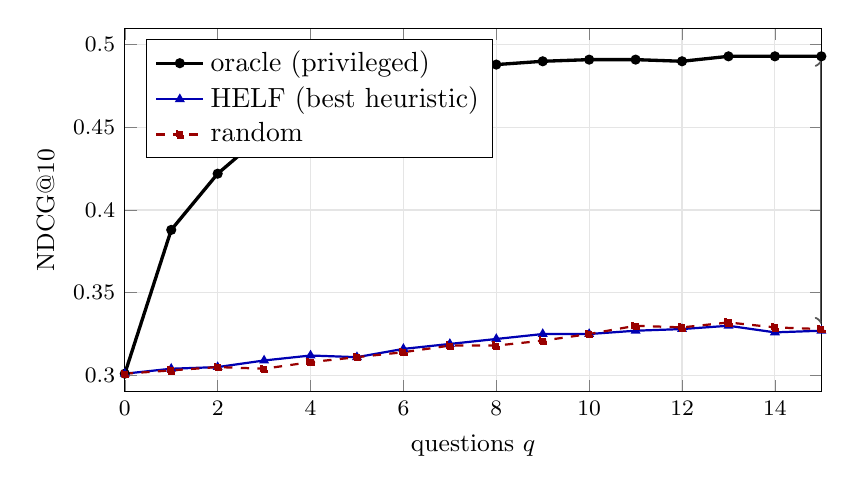
\begin{tikzpicture}
\begin{axis}[width=0.86\textwidth,height=6.2cm,xlabel={questions $q$},ylabel={NDCG@10},
  xmin=0,xmax=15,ymin=0.29,ymax=0.51,legend pos=north west,legend cell align=left,
  grid=major,grid style={gray!20},tick label style={font=\footnotesize},label style={font=\small}]
\addplot[very thick,mark=*,mark size=1.2pt,color=black] coordinates {
 (0,0.301)(1,0.388)(2,0.422)(3,0.446)(4,0.460)(5,0.468)(6,0.476)(7,0.482)(8,0.488)(9,0.490)(10,0.491)(11,0.491)(12,0.490)(13,0.493)(14,0.493)(15,0.493)};
\addlegendentry{oracle (privileged)}
\addplot[thick,mark=triangle*,mark size=1.3pt,color=blue!70!black] coordinates {
 (0,0.301)(1,0.304)(2,0.305)(3,0.309)(4,0.312)(5,0.311)(6,0.316)(7,0.319)(8,0.322)(9,0.325)(10,0.325)(11,0.327)(12,0.328)(13,0.330)(14,0.326)(15,0.327)};
\addlegendentry{HELF (best heuristic)}
\addplot[thick,dashed,mark=square*,mark size=1.1pt,color=red!60!black] coordinates {
 (0,0.301)(1,0.303)(2,0.305)(3,0.304)(4,0.308)(5,0.311)(6,0.314)(7,0.318)(8,0.318)(9,0.321)(10,0.325)(11,0.330)(12,0.329)(13,0.332)(14,0.329)(15,0.328)};
\addlegendentry{random}
\draw[<->,gray!70!black,thick] (axis cs:15,0.331) -- (axis cs:15,0.491)
  node[midway,right,font=\footnotesize,align=left,xshift=-1pt]{selection\\headroom\\$\approx{+}0.16$};
\end{axis}
\end{tikzpicture}
\caption{The selection-headroom gap on the calibrated instrument (item questions, held-out, 150 users, common
$q0=0.301$). A privileged oracle that greedily picks the next item nearly doubles NDCG@10 ($0.30\!\to\!0.49$, with
$+0.09$ from a single question), while the best classical heuristic (HELF) and \emph{random} are indistinguishable
($\approx0.33$). Existing methods capture almost none of a large, reachable-in-principle headroom---the prize a
learned policy must pursue.}
\label{fig:headroom}
\end{figure}

\subsection{Where the headroom is \emph{not}: attributes and naked LLMs}\label{sec:notheadroom}
Two further baselines test whether the selection headroom can be reached by other means than item questions. Both are
\emph{bounded by their own oracles}, so the negatives are rigorous rather than anecdotal.

\textbf{Attribute elicitation has a low ceiling.} We ask genres and Tag-Genome concepts as pseudo-items (factor $=$
taste-space centroid of the attribute's films; answer $=$ leakage-free profile affinity). Even a privileged oracle
that greedily picks the best attribute to reveal lifts NDCG@10 only to $0.332$ ($+0.031$ over the $0.301$ baseline:
genres $+0.025$, concepts $+0.012$), versus the \emph{item} oracle's $0.485$ ($+0.184$); realisable attribute askers
(random, popularity, affinity) move $\le\!+0.007$ (Table~\ref{tab:askers}). The cause is structural and shows at the
oracle level, so it is neither the answer model nor the selector: an attribute is a \emph{coarse direction} (the mean
of hundreds of films), which can localise a user to a broad region but cannot pinpoint specific held-out items, whereas
an item is a precise point. This bounds \emph{every} attribute-elicitation method (EAR/SCPR/UNICORN/PEBOL): none can
exceed $+0.031$ here, so we do not implement them---the oracle already settles the question.

\textbf{A naked LLM asker does not beat random.} A cached \textsc{gpt-4o-mini} asker chooses the next film to ask about
from a fixed menu, given the dialogue so far; we fold the user's true (leakage-free) answer. With a faithful,
adaptive prompt (use the answers, pivot when a title is unseen, prefer divisive over famous films) it reaches only
$0.283$ at $q6$ ($-0.022$), \emph{below} random ($+0.005$) and far below the menu oracle ($+0.180$). The LLM selects
plausibly-divisive titles from world knowledge, but world knowledge is not collaborative informativeness: it has no
access to which items separate users in \emph{this} catalogue's latent geometry, which is what determines an item's
value as a question. (A larger model or a dedicated LLM-RS planner is left to the companion work.)

\begin{table}[h]\centering\small
\begin{tabular}{lcc}
\toprule
selector ($q0\!\to\!q_T$, NDCG@10) & realisable & oracle ceiling\\
\midrule
item elicitation & $0.305\to0.33$ ($+0.025$) & $\mathbf{0.49}$ ($\mathbf{+0.18}$)\\
attribute (genre$+$concept) & $0.30\to0.31$ ($\le\!+0.007$) & $0.33$ ($+0.031$)\\
\quad genres only / concepts only & --- & $+0.025$ / $+0.012$\\
naked LLM asker (\textsc{gpt-4o-mini}) & $0.30\to0.28$ ($-0.022$) & $0.48$ ($+0.18$)\\
\bottomrule
\end{tabular}
\caption{Realisable elicitation vs.\ its oracle ceiling, by channel. Items have a large reachable-in-principle
headroom that no realisable method here captures (heuristics $\approx$ random, \S\ref{sec:answermodel}; LLM $<$ random);
attributes have a \emph{low} ceiling even with an oracle. The selection-headroom gap is therefore an item-question
problem, and an open one---the target of the learned policy.}
\label{tab:askers}
\end{table}

\section{Discussion}\label{sec:disc}

\subsection{Reframing the earlier negative result}
A long prior effort (Appendix~\ref{app:saga}; E1--E13) concluded no realizable policy beats popularity on dense ML
cold-start. We now understand this as an artifact of a \emph{frozen} instrument plus a non-standard NDCG and a
pure-personalization scorer. A recommender frozen on popularity-style interviews cannot convert elicited
information into a better ranking, so every policy collapses to popularity. With a recommender that genuinely
ingests answers, elicitation beats popularity by ${\sim}{+}20\%$ NDCG / ${+}40\%$ Recall.

\subsection{Ours vs.\ adopted}
\emph{Adopted (cited, not claimed):} RMVA seeds, ridge fold-in, the EAR additive scorer, the EDDI acquisition
principle, the Koren bias$+$factor structure, Wolpertinger's continuous mechanism. \emph{Ours:} the
\emph{conjunction}---one shared space serving as both a fold-in recommender over an arbitrary mix of items and open
concepts and the action space of a continuous policy---plus the empirically-grounded floor$+$residual$+$confidence
design, the $D$-optimal seed/recommender coupling, and the acceptance suite.

\subsection{Relationship to bot-play}
The bot-play framework (Makarova et al.\ 2024) trains a questioner by self-play with a per-turn reward equal to the
reduction in the recommender's loss. Empirically (Appendix~\ref{app:saga}) the trained policy collapses to a
near-static playlist: its distinctiveness is the self-play \emph{training} mechanism, not adaptive behaviour, and
under audit it is functionally a static interview. CASPER--U keeps bot-play's decision-focused reward but replaces
(i) the frozen item-only recommender with the unified fold-in instrument, and (ii) the discrete-item policy with a
continuous-semantic-space policy---addressing the two reasons the original collapsed.

\subsection{Threats to validity}
\textbf{Reproducibility:} we anchored to a published baseline number and treat unreproducible method gains (DRE's
neural decoder) as honest negatives. \textbf{Metric choice:} NDCG@10 is blockbuster-biased; we therefore lead with
Recall@10 and report both. \textbf{Single dataset:} the instrument is shown on ML-1M; attribute mechanism
additionally on LastFM (R2). \textbf{Open concepts:} transfer is only partial (\S\ref{sec:concepts})---a controlled
no-genre-word test with a title-only ablation shows success for title-recoverable concepts that form taste clusters
and failure for plot-level themes absent from the item text; the binding limitation is the thin item text
(title$+$genres), and enriching it with plot synopses is the concrete remedy, not a change to the mechanism. \textbf{Simulator realism:} answers are oracle-derived from ground-truth ratings;
LLM-simulated noise is future work. \textbf{Leakage:} the blend weight is tuned on a disjoint validation split and
reported once on test; genre ``confirmed preferences'' are high-level facts, not held-out items.

\section{Roadmap}\label{sec:roadmap}
\textbf{S3 (items$+$attributes complete; open concepts partial, \S\ref{sec:concepts}):} genre attributes are fully
demonstrated; the SBERT adapter transfers open concepts only partially (well when the concept is recoverable from
the title and forms a taste cluster, poorly for plot-level themes absent from the thin item text). Enriching item
descriptions with plot synopses is the concrete next step to complete open-concept support.
\textbf{S4:} the full elicitation baseline panel on the fixed instrument (random, popularity, RMVA, Golbandi tree,
greedy information-gain, SCPR/UNICORN-style discrete DQN, PEBOL/Thompson). \textbf{S5:} the continuous-action
(Wolpertinger-style) policy over the unified space---the thesis contribution---evaluated against S4 and a
discrete-action policy. \textbf{S6:} naked-LLM askers, quantifying prompt-only LLM elicitation (RQ3).

\section{The frozen-instrument saga (E1--E13)}\label{app:saga}
Heuristics, behaviour cloning, RLOO, belief-conditioned actors, BC$+$RL, residual policy learning, and
DQfD/POfD-style oracle-pull were tried against a \emph{frozen} instrument across ML-100k and ML-1M, two metrics
(NDCG, serendipity), with validation-stopping and a guaranteed popularity floor. All converged to popularity. The
decisive insight (E14) was that the binding constraint was the frozen recommender, not the policy---motivating
CASPER--U. Full log archived in \texttt{archive/CASPER\_EXPERIMENTS\_E1-E14\_archived.md}.

\section{Live scripts}\label{app:scripts}
\texttt{mf\_foldin.py} (R1/S1), \texttt{ear\_lastfm.py} (R2), \texttt{eddi\_replicate.py} (R3),
\texttt{instrument\_u.py} (S2), \texttt{instrument\_u\_attr.py} (S3), \texttt{instrument\_u\_sanity.py}
(interpretable checks), \texttt{golbandi\_tree.py} (adaptive-tree RMSE replication), \texttt{dre\_faithful.py}
(DRE baseline reproduction). Live ledger: \texttt{RESULTS.md}.

